\documentclass[border=2pt]{standalone}
\usepackage{tikz}
\usetikzlibrary{through}
\usetikzlibrary{calc}
\usetikzlibrary{intersections}


\begin{document}
    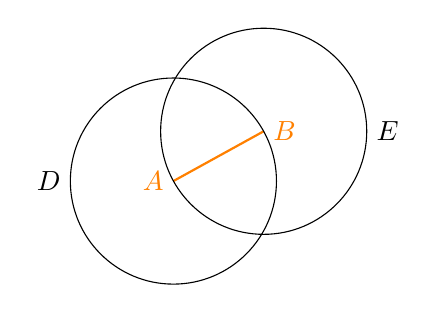
\begin{tikzpicture}
        \coordinate [label=left:$\textcolor{orange}{A}$] (A) at ($(0, 0)+0.1*(rand, rand)$);
        \coordinate [label=right:$\textcolor{orange}{B}$] (B) at ($(1.25, 0.5)+0.1*(rand, rand)$);
        \draw [orange, thick] (A) -- (B);

        \node (D) [draw, circle through=(B), label=left:$D$, name path=D] at (A) {};
        \node (E) [draw, circle through=(A), label=right:$E$, name path=E] at (B) {};

        \path [name intersections={of=D and E}];
    \end{tikzpicture}
\end{document}